% Descripción de estos servidores 
Un servidor de correo es una aplicacion de red de computadoras ubicada en un servidor de Internet, para prestar servicio de correo electrónico. De forma predeterminada, el protocolo estándar para la transferencia de correos entre servidores es el Protocolo Simple de Transferencia de Correos (SMTP).
\subsubsection{Instalación del servidor}
En este caso se utilizó el servidor SMTP llamado Postfix. Los pasos para su instalación son los siguientes:
\begin{figure}[!htbp]
	\hypertarget{fig:instalacionSMTP}{\hspace{1pt}}
	\begin{center}
		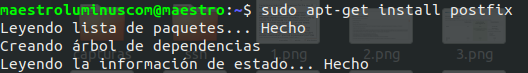
\includegraphics[width=0.7\textwidth]{desarrollo/tarea2/img/instalacionSMTP.png}
		\caption{Comando para instalar un servidor SMTP llamado Postfix}
		\label{fig:instalacionSMTP}
	\end{center}
\end{figure}
\pagebreak
\begin{figure}[!htbp]
	\hypertarget{fig:reiniciarSMTP}{\hspace{1pt}}
	\begin{center}
		
\includegraphics[width=0.7\textwidth]{desarrollo/tarea2/img/reiniciarSMTP.png}
		\caption{Comando para reiniciar el servicio SMTP}
		\label{fig:reiniciarSMTP}
	\end{center}
\end{figure}